\documentclass[12pt,prb,aps,epsf]{article}
\usepackage[utf8]{inputenc}
\usepackage{amsmath}
\usepackage{amsfonts}
\usepackage{amssymb}
\usepackage{graphicx} 
\usepackage{latexsym} 
\usepackage[toc,page]{appendix}
\usepackage{listings}
\usepackage{xcolor}
\usepackage{soul}
\usepackage[T1]{fontenc}
\usepackage{amsthm}
\usepackage{mathtools}
\usepackage{setspace}
\usepackage{array,multirow,makecell}
\usepackage{geometry}
\usepackage{textcomp}
\usepackage{float}
%\usepackage{siunitx}
\usepackage{cancel}
%\usepackage{tikz}
%\usetikzlibrary{calc, shapes, backgrounds, arrows, decorations.pathmorphing, positioning, fit, petri, tikzmark}
\usepackage{here}
\usepackage{titlesec}
%\usepackage{bm}
\usepackage{bbold}
\geometry{hmargin=2cm,vmargin=2cm}

\begin{document}
	
	\title{MP 16 Milieux magnétiques}
		\author{Naïmo Davier}
		\date{Agrégation 2019}
		
	\maketitle
	
	\tableofcontents
	
	\pagebreak
	
\subsection{Introduction}
Définition susceptibilité. Étude ici des ferro et para seulement correspondant au cas d'une susceptibilité positive.	
\section{Susceptibilité d'une solution de $FeCl_3$}	
\textbf{Quaranta Tome IV l'électricité} + site d'Étienne thibierge\\
	
On place un tube en U, empli d'une solution de $FeCl_3$ à 50\% en masse, dans une zone de fort gradient de champ magnétique, généré à l'aide d'un électroaimant.\\

On a $\vec{M} = \chi_{sol}\vec{B}$ et donc 
\begin{eqnarray}
\vec{F} = -(\vec{M}.\vec{\nabla})\vec{B} = -\vec{\nabla}\phi 
\end{eqnarray}
où $\phi = \frac{\chi_{sol}B^2}{2\mu_0}$.\\

En appliquant le théorème de Bernoulli en prenant en compte le potentiel lié à la pression magnétique donné ci dessus on obtient que la hauteur $h$ dont le ménisque de la solution va varier est telle que 
\begin{eqnarray}
\rho_{sol}gh = \frac{\chi_{sol} }{2\mu_0} (B^2(A)-B^2(B))
\end{eqnarray}

On a une solution à 50\% en masse, ce qui permet d'établir 
\begin{eqnarray}
\chi_{FeCl_3} = \frac{2\rho_{FeCl_3}\chi_{sol}}{\rho_{sol}}
\end{eqnarray}
et ainsi 
\begin{eqnarray}
B^2(A)- B^2(B) = \frac{4\rho_{FeCl_3}g\mu_0}{\chi_{FeCl_3}}h
\end{eqnarray}
où on a $\rho_{FeCl_3} = 2800$ kg.m$^{-3}$.\\

On mesure $h$ en fonction de la différence de potentiel magnétique, pour être plus précis on réalise une projection du tube à l'aide d'une lentille de focale 15cm afin de mesurer $h$ qui est de l'ordre du mm. On mesure le grandissement de notre montage à l'aide d'une mire placée dans le même plan que le tube.\\ On trace ensuite 
\begin{eqnarray}
B^2(A) - B^2(B) = f(h)
\end{eqnarray}
et on fait une régression affine pour en déduire une mesure de $\chi_{FeCl_3}$. On pourra comparer cette valeur à la valeur tabulé qui est de $\chi_{FeCl_3}^{tab} = 3,3.10^{-3}$.\\

On a vu une méthode permettant de mesurer la susceptibilité magnétique d'une solution, on va maintenant en voir une application.
	
	
\section{Effet Faraday}
Voir la \textbf{Notice effet faraday}\\

On envoie un faisceau laser polarisé rectilignement à travers un tube de Flint qui est soumis à un champ magnétique car il est placé au centre d'une bobine.	On place en sortie un analyseur orienté à 45° par rapport au polariseur et on relève la puissance lumineuse en sortie à l'aide d'un puissancemètre, en fonction du courant $I$ imposé à la bobine.\\

On a dans la pratique un angle de déviation $\beta = VLB = V\alpha I$ où $\alpha = 4,6\pm0,16 \, .10^{-3}$ T/A est donné par le constructeur, et V est la constante de Verday pour le flint : c'est ce que l'on veut mesurer ici.\\

La loi de mallus nous donne, à 45° que le facteur de transmission vaut 
\begin{eqnarray}
T = \cos^2\theta &\Rightarrow& \frac{dT}{d\theta}(\theta=45^o) = 1\\
&\Rightarrow& p = \frac{dT}{dI} = \pm \frac{d\theta}{dI} = V\alpha
\end{eqnarray}

On trace donc ici $T=\frac{P_{45}-P_{min}}{P_{max}-P_{min}}=f(I)$ puis on fait une régression affine afin d'évaluer le coefficient directeur $p$, on en déduit finalement 
\begin{eqnarray}
V = \frac{p}{\alpha}
\end{eqnarray}
On pourra alors comparer le résultat obtenu à la valeur tabulé pour le flint qui est de 14,1.

\section{Caractérisation d'un ferromagnétique}
Fait dans le \textbf{quaranta tome IV Électricité}

\subsection{Courbe de première aimantation}
On réalise le circuit suivant avec un générateur courant tension délivrant $V_e$, et un potensiostat $R$ conçut pour supporter de grosses intensités.\\
\begin{figure}[h]
	\centering \includegraphics[width=10cm]{circuit}
\end{figure}

Les tensions $V_R$ et celle aux bornes de la seconde bobine sont envoyées vers latis-pro. $V_R$ nous donne l'intensité traversant le primaire et nous donne ainsi l'expression du champ $H = \frac{N_1 I}{l} = \frac{N_1 V_R}{Rl}$ où $l$ est la longueur moyenne de la boucle formée par le ferromagnétique. La tension aux bornes de la seconde bobine nous donne la force électromotrice $e$ générée par le flux total de champ magnétique à travers la bobine, on a donc, en notant $S$ la surface d'une spire 
\begin{eqnarray}
e = \frac{d\Phi}{dt} = N_2\frac{d\phi}{dt} = N_2 S \frac{dB}{dt}
\end{eqnarray}
et on en déduit ainsi une mesure de $B$ selon
\begin{eqnarray}
B(t) = \frac{1}{N_2S} \int_0^t  e(\tau)\;d\tau
\end{eqnarray}
en réalisant une intégration numérique grâce à Latis pro.\\

On tracera alors $B(H)$ ou au choix $M(H) = \frac{B(H)}{\mu_0}-H$ en augmentant progressivement $I$ jusque qu'au courant maximal toléré par la première bobine ($\simeq 2$ A) pour obtenir la courbe de première aimantation.
\begin{figure}[h]
	\centering 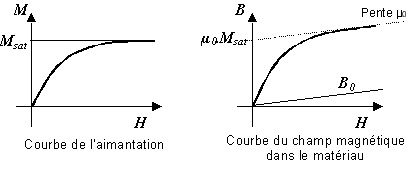
\includegraphics[width=12cm]{1ere_aimantation}
\end{figure}

\subsection{Cycle d'hystérésis}
La démarche est la même que pour obtenir la courbe de première aimantation sauf que cette fois on place un Générateur pour lequel on peut régler le pourcentage de la puissance transmise par le secteur, on se place donc à une tension max telle que l'intensité n'excède pas l'intensité max supportée par la première bobine. On réalise ensuite une acquisition similaire à la précédente, mais sur un temps plus court : la tension délivrée oscillant à 50 Hz il suffit de prendre un temps d'acquisition de plus de 20 ms pour avoir un cycle complet. Attention la tension $e$ aux borne de la seconde bobine peut facilement excéder les 10 V, on placera donc dans ce cas un pont diviseur de tension afin de ne pas faire saturer latis pro.\\

Pour calculer la perte fer et ainsi caractériser le ferro on calculera l'intégrale 
\begin{eqnarray}
\int B(H) dH = 2\int_0^{T/2} B(t)\frac{dH}{dt} dt
\end{eqnarray}
en choisissant les bornes de l'intégrale de telle sorte à intégrer sur une demie période.

\section*{Questions}
Pouvez retrouver l'expression donnée pour $\chi_{FeCl_3}$ ?\\

Pourquoi place t'on l'analyseur à 45° ?\\
Pour linéariser la transmitance.\\

Quels sont les modes propres de polarisation qui se propagent dans le flint ?\\
polarisations circulaires gauche et droites, elles ne se déplacent pas à la même vitesse (indices optiques perçus différents) : la somme des deux est alors une rectiligne qui tourne.\\

Connaissez vous d'autre type d'effet faisant tourner la polarisation ?\\
Pouvoir rotatoire d'une solution qui est anisotrope : les polarisations droites et gauche voient des indices optiques différents.\\

Comment cet effet varie t-il avec la longueur d'onde ?\\
Lorsque la longueur d'onde augment l'effet diminue.




\end{document}